\documentclass[12pt, a4paper]{article}

\usepackage{amsmath}
\usepackage{bbm}
\usepackage{amsfonts}
\usepackage{graphicx}
\usepackage{pdfpages}
\usepackage[titletoc, title]{appendix}
\usepackage{hyperref}
\hypersetup{
    colorlinks=true,
    linkcolor=blue,
    filecolor=magenta,      
    urlcolor=cyan,
}


\def\va{\boldsymbol{a}}
\def\vb{\boldsymbol{b}}
\def\vc{\boldsymbol{c}}
\def\vh{\boldsymbol{h}}
\def\vs{\boldsymbol{s}}
\def\vw{\boldsymbol{w}}
\def\vx{\boldsymbol{x}}
\def\vy{\boldsymbol{y}}
\def\vz{\boldsymbol{z}}
\def\v1{\boldsymbol{1}}

\def\vI{\boldsymbol{I}}
\def\vR{\boldsymbol{R}}
\def\vU{\boldsymbol{U}}
\def\vV{\boldsymbol{V}}
\def\vW{\boldsymbol{W}}
\def\vX{\boldsymbol{X}}
\def\vY{\boldsymbol{Y}}

\def\vtheta{\boldsymbol{\theta}}

\def\rmx{\mathrm{x}}

\def\vrmx{\boldsymbol{\mathrm{x}}}
\def\vrmy{\boldsymbol{\mathrm{y}}}
\def\vrmX{\boldsymbol{\mathrm{X}}}
\def\vrmY{\boldsymbol{\mathrm{Y}}}

\def\E{\mathbb{E}}
\def\X{\mathbb{X}}
\def\R{\mathbb{R}}

\def\st{\textit{s.t.}}

\DeclareMathOperator*{\relu}{ReLU}
\DeclareMathOperator*{\argmax}{arg\,max}
\DeclareMathOperator*{\argmin}{arg\,min}
\DeclareMathOperator*{\softmax}{softmax}
\DeclareMathOperator*{\diag}{diag}

\newcommand{\egva}[1]{\boldsymbol{a}^{(#1)}}
\newcommand{\egvb}[1]{\boldsymbol{b}^{(#1)}}
\newcommand{\egvc}[1]{\boldsymbol{c}^{(#1)}}
\newcommand{\egvh}[1]{\boldsymbol{h}^{(#1)}}
\newcommand{\egvo}[1]{\boldsymbol{o}^{(#1)}}
\newcommand{\egvs}[1]{\boldsymbol{s}^{(#1)}}
\newcommand{\egvx}[1]{\boldsymbol{x}^{(#1)}}
\newcommand{\egvy}[1]{\boldsymbol{y}^{(#1)}}
\newcommand{\egvU}[1]{\boldsymbol{U}^{(#1)}}
\newcommand{\egvV}[1]{\boldsymbol{V}^{(#1)}}
\newcommand{\egvW}[1]{\boldsymbol{W}^{(#1)}}
\newcommand{\egh}[1]{h^{(#1)}}
\newcommand{\ego}[1]{o^{(#1)}}
\newcommand{\egx}[1]{x^{(#1)}}
\newcommand{\egy}[1]{y^{(#1)}}
\newcommand{\egL}[1]{L^{(#1)}}
\newcommand{\eghy}[1]{\hat{y}^{(#1)}}
\newcommand{\eghvy}[1]{\hat{\boldsymbol{y}}^{(#1)}}

\newcommand{\expect}[3]{\mathbb{E}_{#1 \sim #2} \left[ #3 \right]}
\newcommand{\dkl}[2]{D_{\mathrm{KL}}(#1 \Vert #2)}
\newcommand{\condiP}[3]{P(#1 \mid #2;#3)}
\newcommand{\condip}[3]{p(#1 \mid #2;#3)}
\newcommand{\ND}[3]{\mathcal{N}(#1;#2,#3)}

\newcommand{\dx}[1]{\frac{\mathrm{d}}{\mathrm{d}x} #1}
\newcommand{\pard}[2]{\frac{\partial #1}{\partial #2}}
\newcommand{\tpard}[2]{\left(\frac{\partial #1}{\partial #2}\right)^\top}


\title{Recurrent Neural Network}
\author{CHEN Si}
\date{}


\begin{document} 


\maketitle
\tableofcontents


\section{Definition}
\begin{center}
    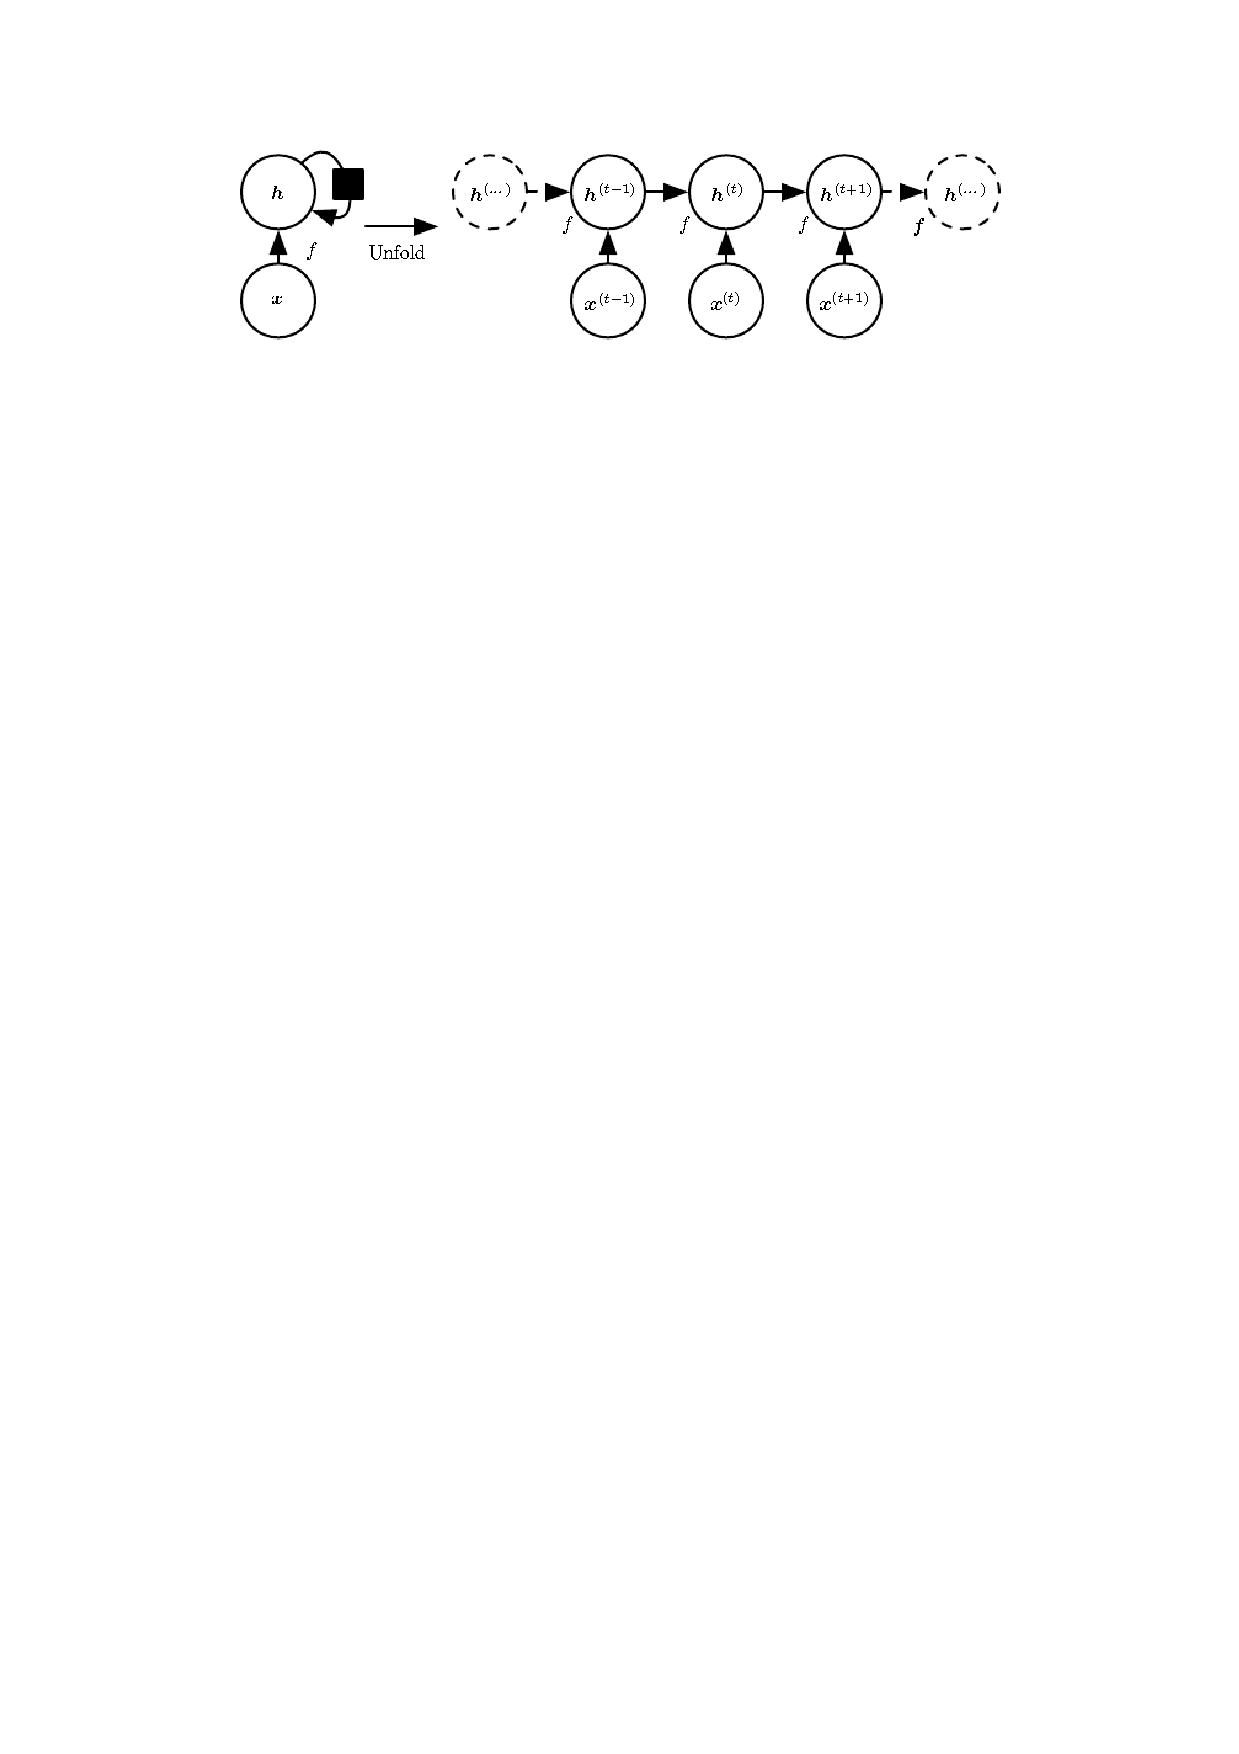
\includegraphics[width=0.9\textwidth]{../imgs/Recurrent_Network_without_Outputs.pdf}
\end{center}
\[
    \egvh{t} = f(\egvh{t-1}, \egvx{t};\vtheta)
\]
\begin{itemize}
    \item Hidden units $\vh$ represents
        \begin{enumerate}
            \item the state of the dynamical system.
            \item lossy summary of the task-relevant aspects of the past sequence of inputs up to $t$, when the recurrent network is trained to perform a task that requires predicting the future from the past.
        \end{enumerate}
    \item Black square indicates that an interaction takes place with a delay of a single time step.
\end{itemize}


\subsection{Motivation}

\paragraph{Dynamical System}
\subparagraph{Unfolded Computational Graph}
\begin{center}
    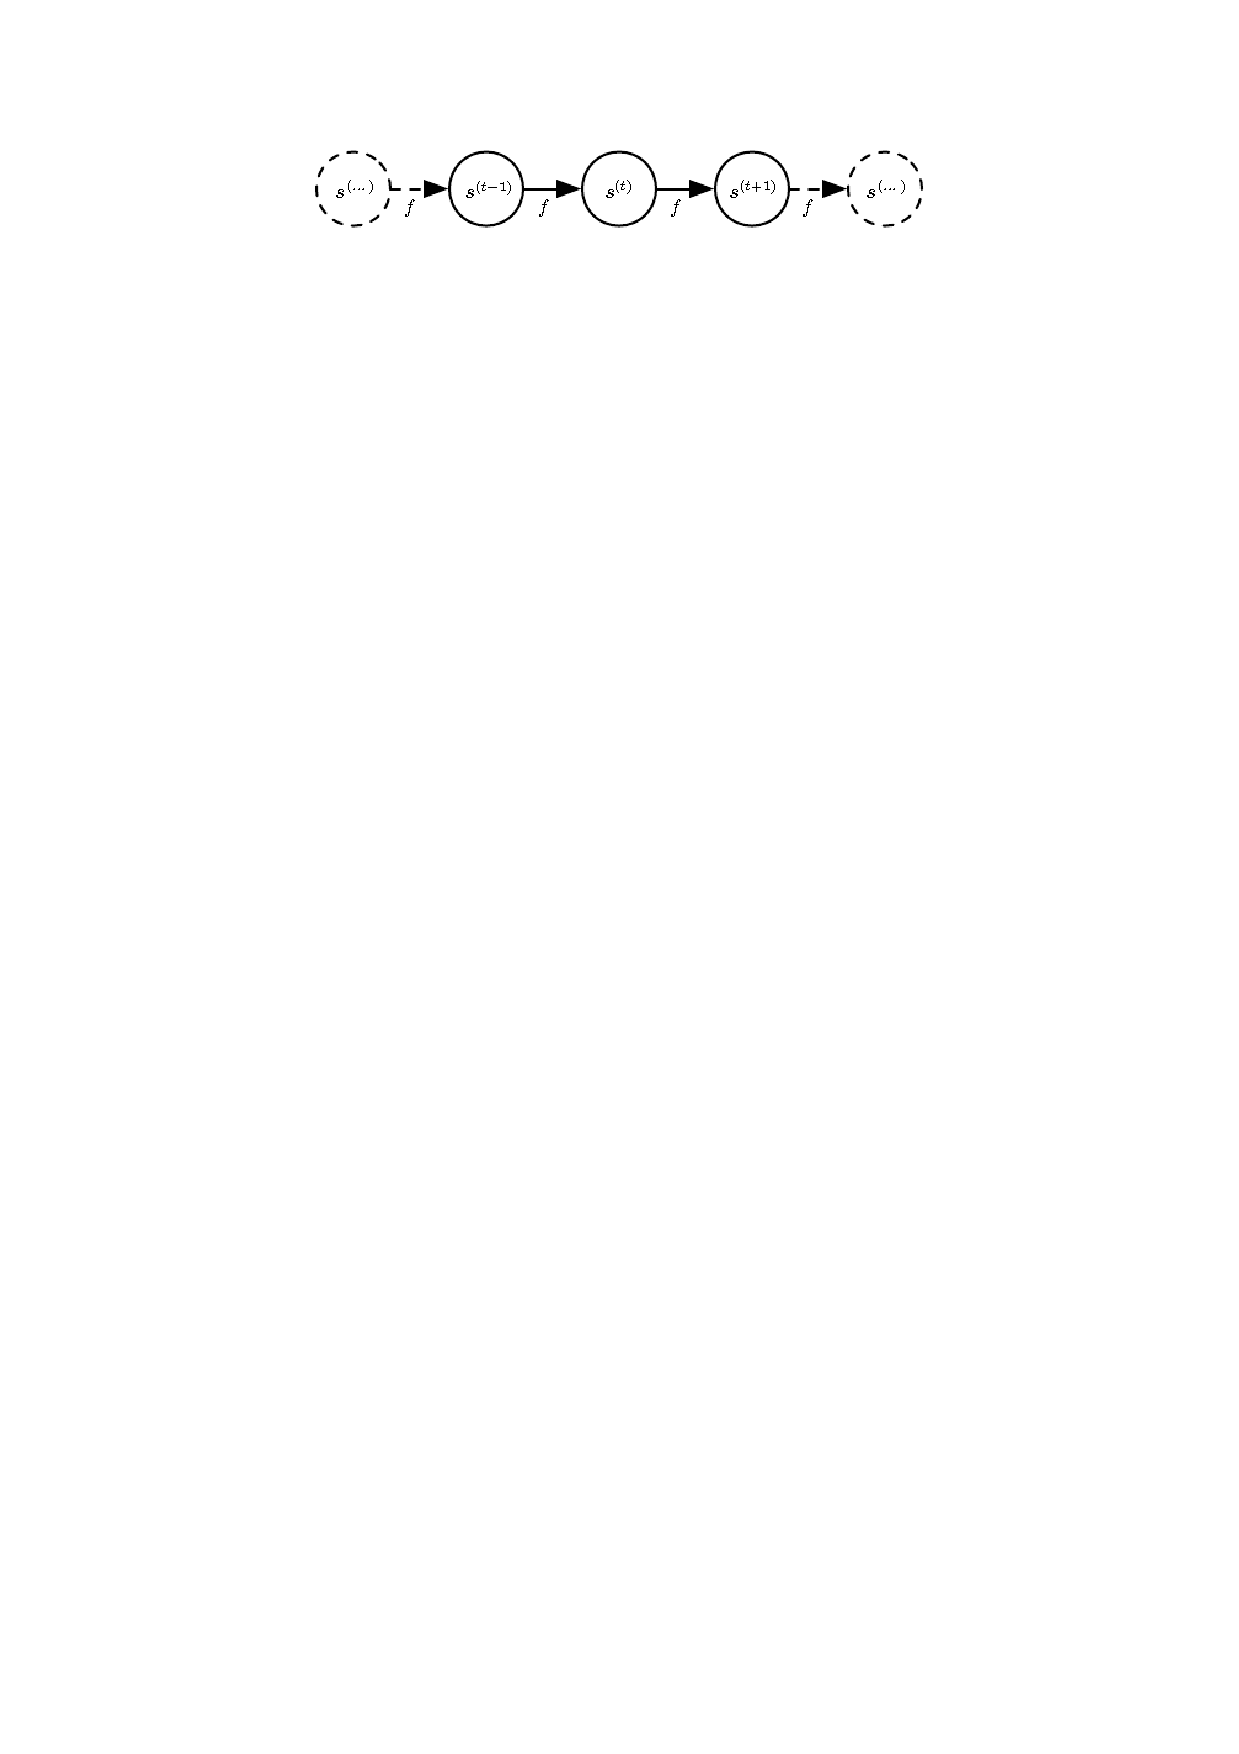
\includegraphics[width=0.8\textwidth]{../imgs/Dynamical_System.pdf}
\end{center}
where $\egvs{t}$ is called the \textbf{state} of the system.
\subparagraph{Recurrent Defintion}
\[
    \egvs{t} = f(\egvs{t-1};\vtheta)
\]
\subparagraph{Unfolded Definition (up to step 3)}
\[
    \begin{split}
        \egvs{3} &= f(\egvs{2};\vtheta)
        \\&= f(f(\egvs{1};\vtheta);\vtheta)
    \end{split}
\]

\paragraph{Dynamical System with External Signal $\egvx{t}$}
\[
    \egvs{t} = f(\egvs{t-1}, \egvx{t}; \vtheta)
\]


\subsection{Advantages}
\begin{enumerate}
    \item Learning just a single model $f$:
        \begin{itemize}
            \item The learned model always has the same input size, regardless of the sequence length.
            \item Parameter sharing: It is possible to use the same transition function $f$ with the same parameters at every time step.
            \item Allows generalization to sequence lengths that does not appear in the training set.
            \item Requires much fewer training examples to estimate.
        \end{itemize}
\end{enumerate}


\subsection{Disadvantages}
\begin{enumerate}
    \item Optimizing the parameters may be difficult, because of the reduced number of parameters.
\end{enumerate}


\subsection{How to determine the length $\tau$}
\begin{enumerate}
    \item Add a special symbol corresponding to the end of a sequence.
    \item Introduce an extra Bernoulli output to the model that represents the decision to either contnue generation or halt generation at each time step. (a more general way)
    \item Add an extra output to the model that predicts the interger $\tau$ itself.
        \[
            P(\egvx{1},\dots,\egvx{\tau}) = P(\tau) P(\egvx{1},\dots,\egvx{\tau} \mid \tau)
        \]
\end{enumerate}


\section{Taxonomy}

\subsection{}
Recurrent networks that produce an output at each time step and have recurrent connections between hidden units.
\begin{equation}
    \begin{split}
        \egva{t} &= \vb + \vW\egvh{t-1} + \vU\egvx{t} \\
        \egvh{t} &= \tanh(\egva{t}) \\
        \egvo{t} &= \vc + \vV\egvh{t} \\
        \eghvy{t} &= \softmax(\egvo{t})
    \end{split}
    \label{rnn_for}
\end{equation}
with a initial state $\egvh{0}$.
\begin{center}
    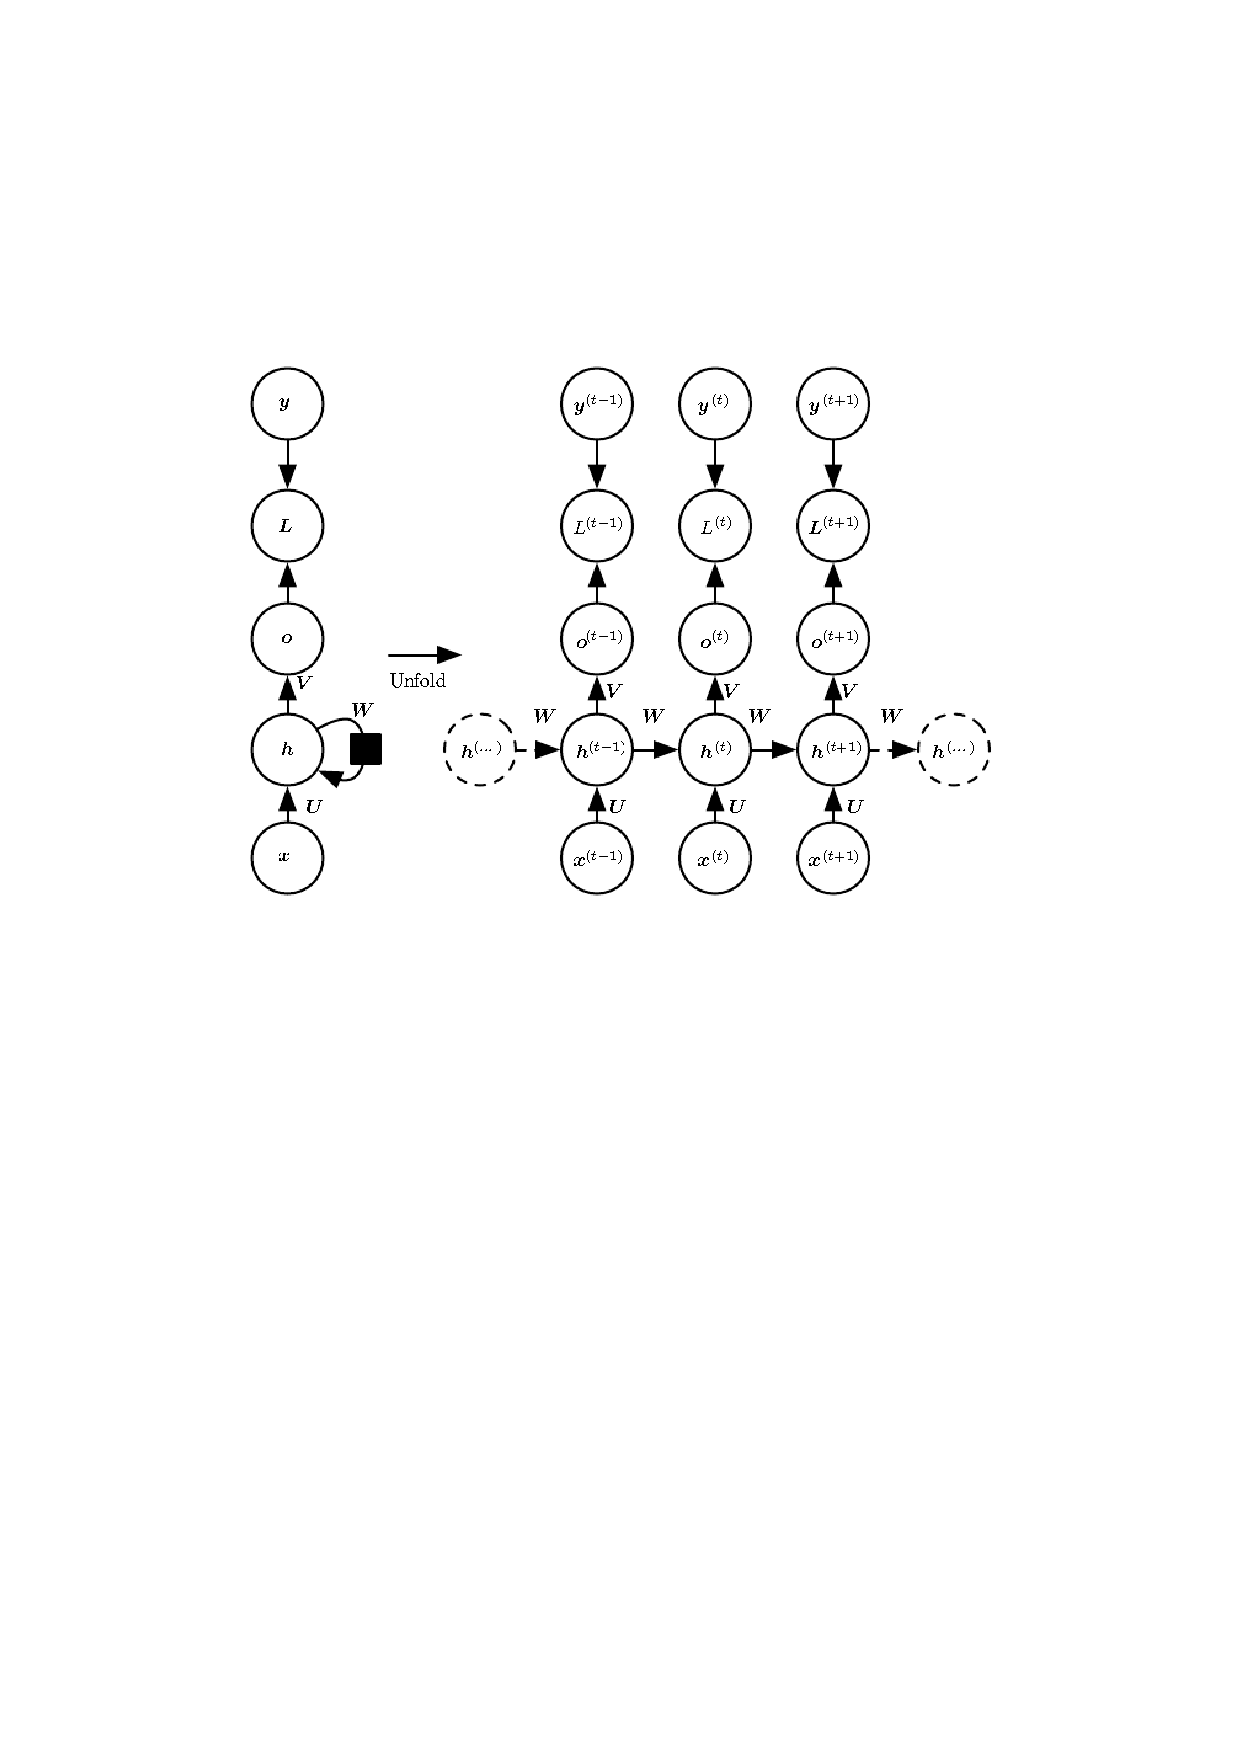
\includegraphics[width=0.9\textwidth]{../imgs/RNN_1.pdf} 
\end{center}

\paragraph{Characteristics}
\begin{itemize}
    \item Maps an input sequence to an output sequence of the same length.
    \item{
        Loss:
        \begin{equation}
            \begin{split}
                & L\left( \{\egvx{1},\dots,\egvx{\tau}\}, \{\egvy{1},\dots,\egvy{\tau}\} \right)
                \\=& \sum_t \egL{t}
                \\=& - \sum_t \log p_\text{model} \left( \egy{t} \mid \{\egvx{1},\dots,\egvx{t}\} \right)
            \end{split}
            \label{rnn_loss}
        \end{equation}
        where $\egL{t}$ is the negative log-likelihood of $\egy{t}$ given $\egvx{1},\dots,\egvx{t}$
        \begin{itemize}
            \item{
                Conditional independence assumption: The conditional distribution 
                \[
                    P( \egvy{1},\dots,\egvy{\tau} \mid \egvx{1},\dots,\egvx{\tau} ) = 
                    \prod_t P(\egvy{t} \mid \egvx{1},\dots,\egvx{t})
                \]
            }
        \end{itemize}
    }
    \item Runtime is $O(\tau)$, memory cost is $O(\tau)$.
    \item Only able to represent distributins in which the $\vy$ values are conditionally independent from each other given the $\vx$ values.
\end{itemize}

\subsection{}
Recurrent networks that produce an output at each time step and have recurrent connections only from the output at one time step to the hidden units at the next time step.
\begin{center}
    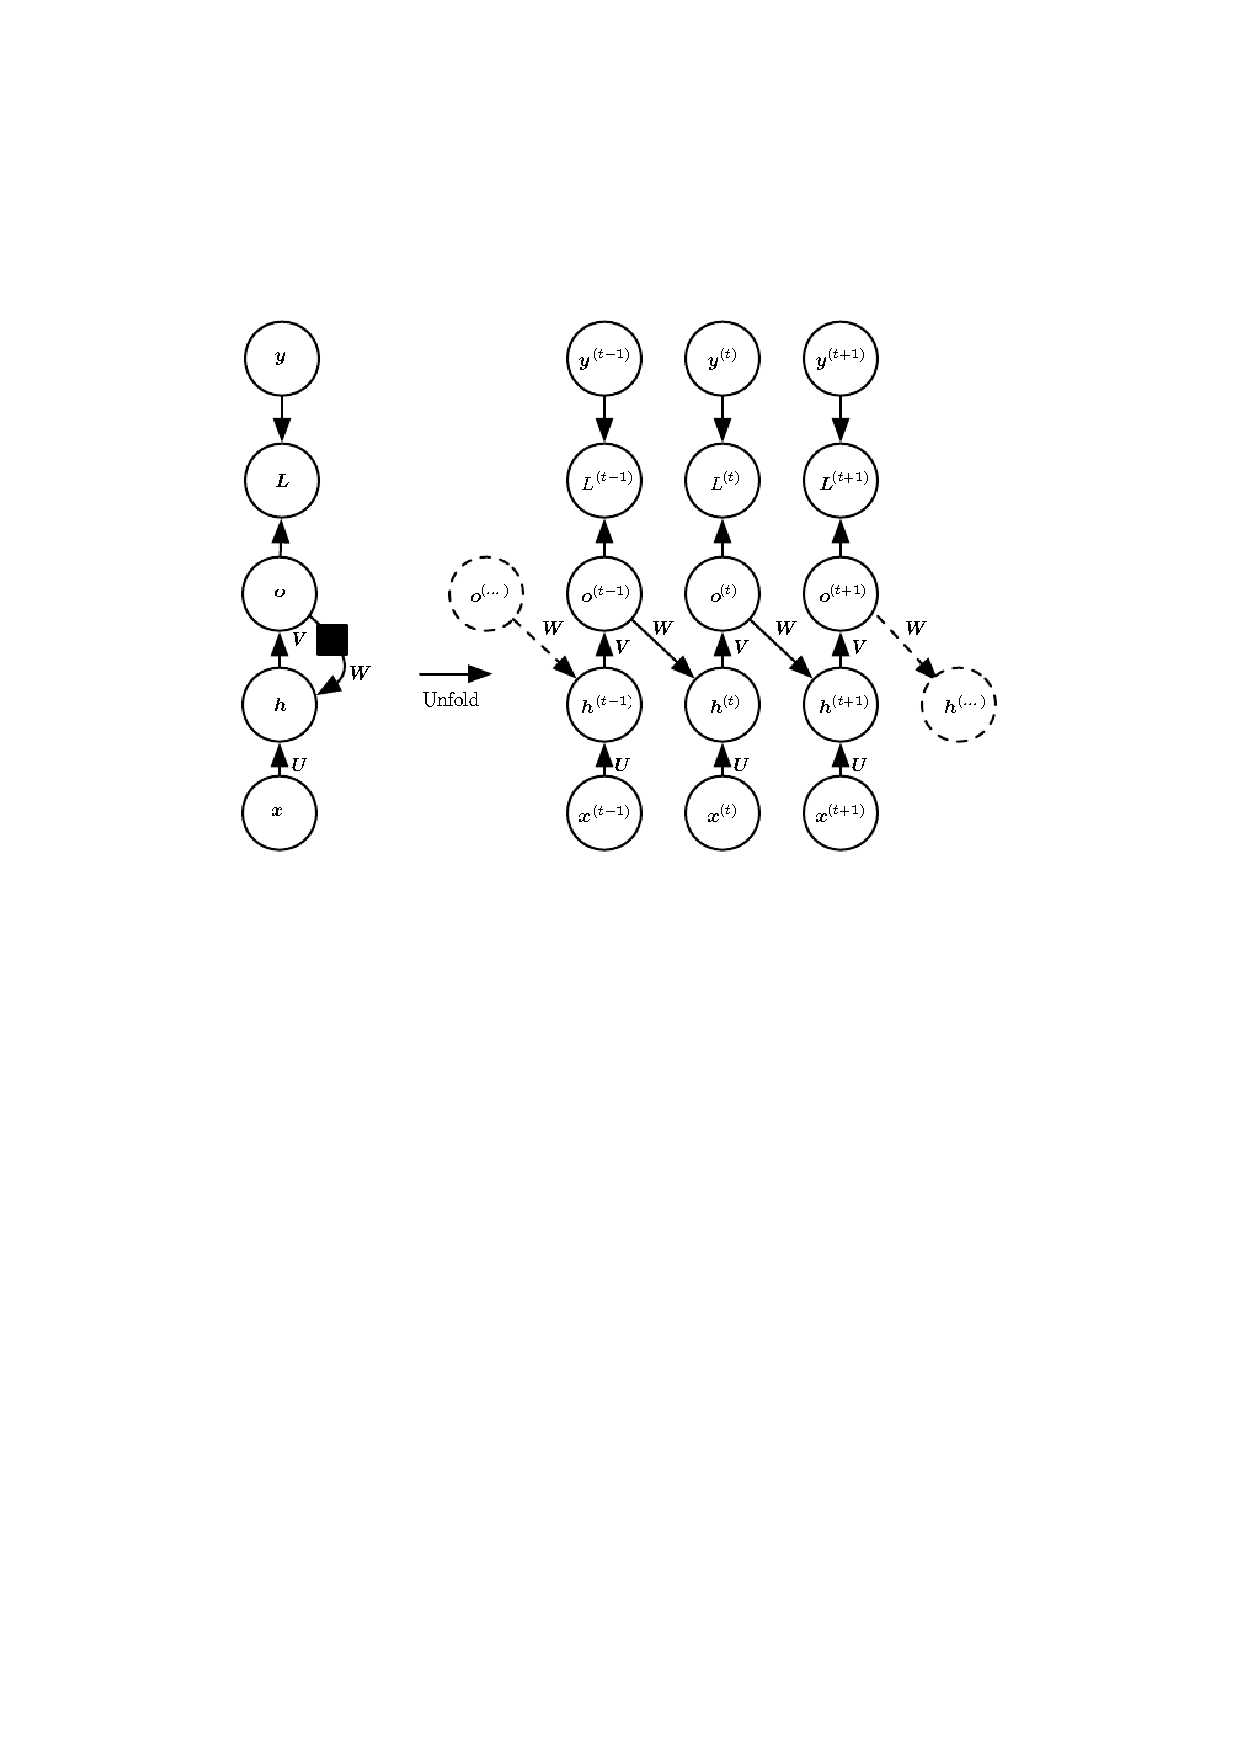
\includegraphics[width=0.9\textwidth]{../imgs/RNN_2.pdf}
\end{center}
\paragraph{Characteristics}
\begin{itemize}
    \item Strictly less powerful because it lacks hidden-to-hidden recurrent connections. (e.g. it connot simulate a universal Turing machine.)
    \item Training can be \textbf{parallelized} because all the time steps are decoupled (the training set provides the ideal value of previous output).
    \item Avoids back-propagation through time.
    \item Teacher forcing:
        For example, for a sequence with two time steps
        \[
            \begin{split}
                &\log p\left( \egvy{1},\egvy{2} \mid \egvx{1},\egvx{2} \right)
                \\=& \log p\left(\egvy{2} \mid \egvy{1},\egvx{1},\egvx{2} \right) + \log p\left( \egvy{1} \mid \egvx{1},\egvx{2} \right)
            \end{split}
        \]
        \begin{center}
            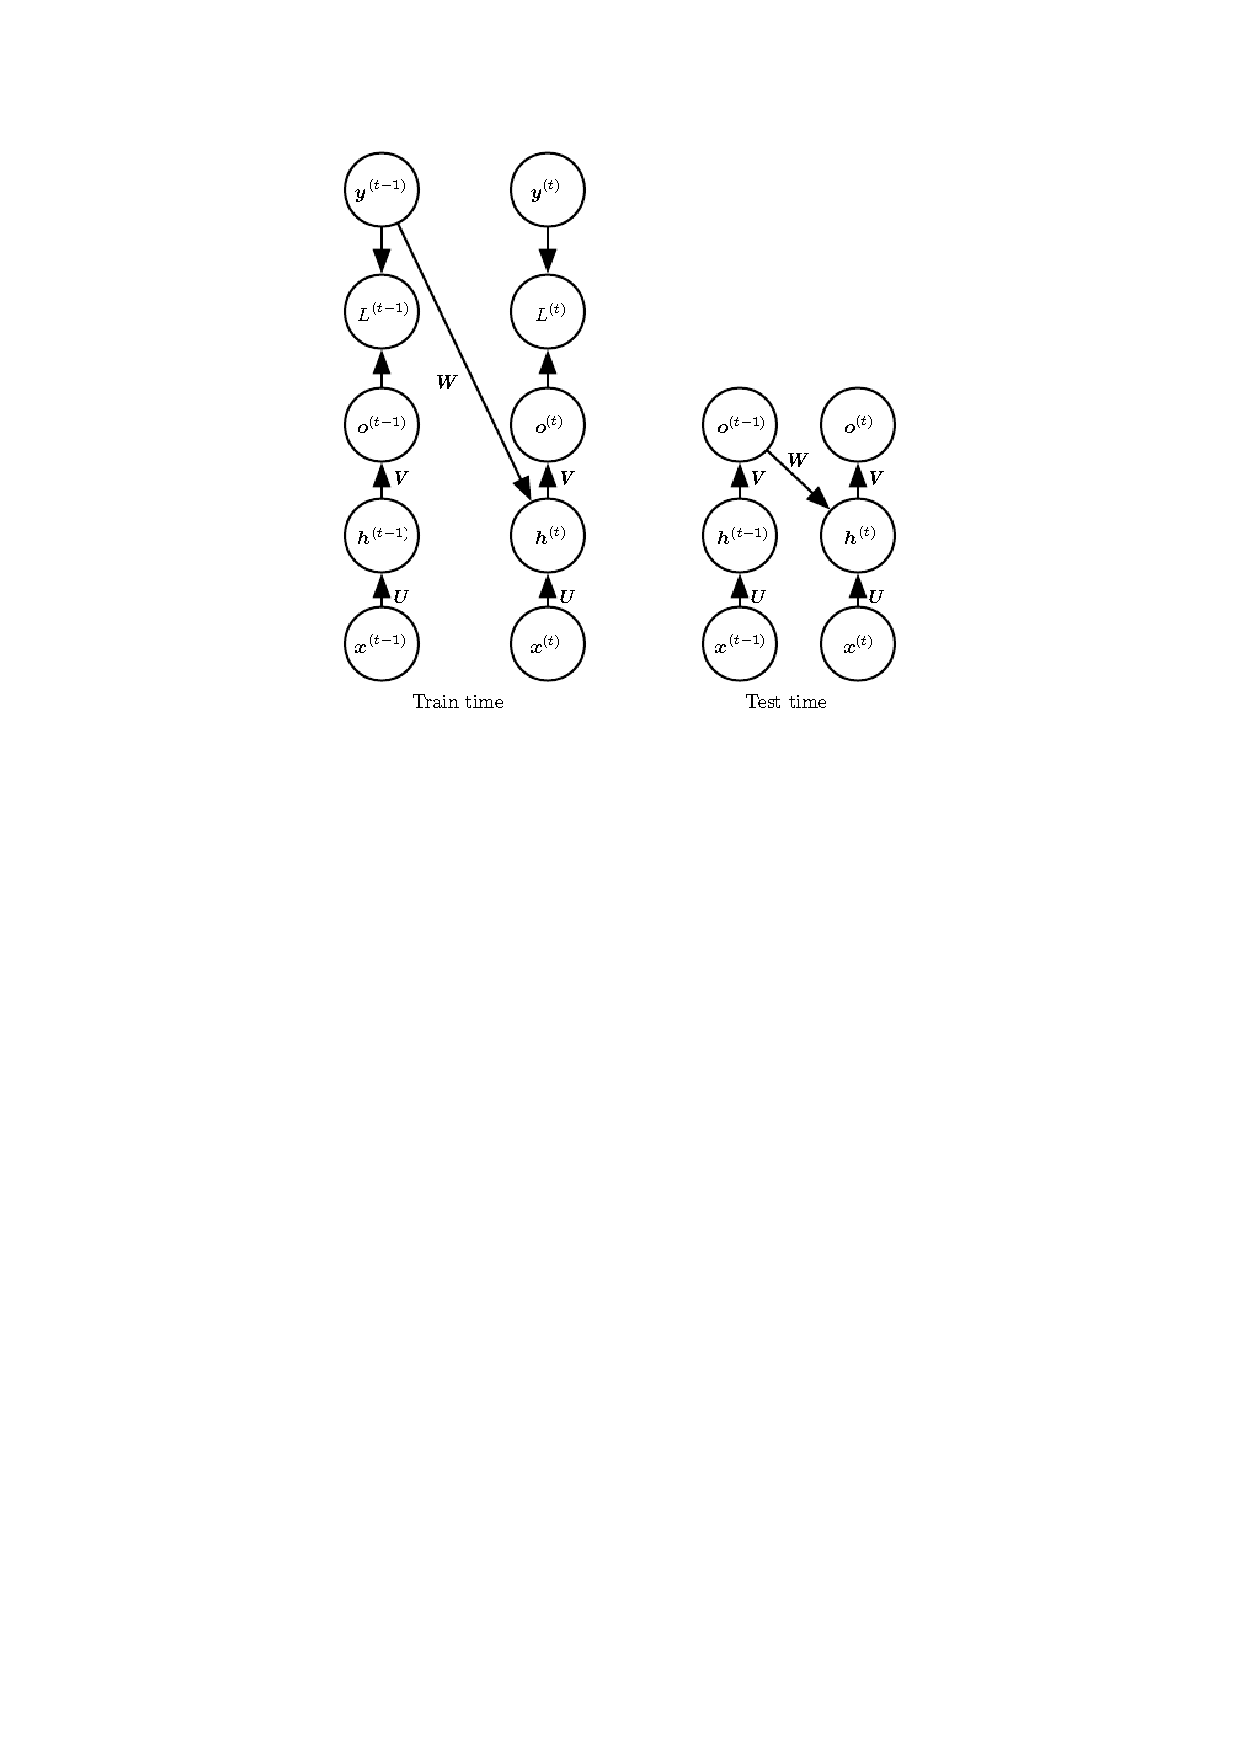
\includegraphics[width=0.7\textwidth]{../imgs/Teacher_Forcing.pdf}
        \end{center}
\end{itemize}
\paragraph{Disadvantages}
\begin{enumerate}
    \item The disadvantages of strict teacher forcing (no BPTT) is that the inputs during training could be quite different from the inputs during testing (\textbf{closed-loop} mode).
        \newline Solutions:
        \begin{enumerate}
            \item Train with both teacher-forced inputs and free-running inputs
            \item Randomly chooses to use generated values or actual data values as input (curriculum learning strategy: gradially use more of the generated values as input).
        \end{enumerate}
\end{enumerate}

\subsection{}
Recurrent networks with recurrent connections between hidden units, that read an entire sequence and then produce a single output.
\begin{center}
    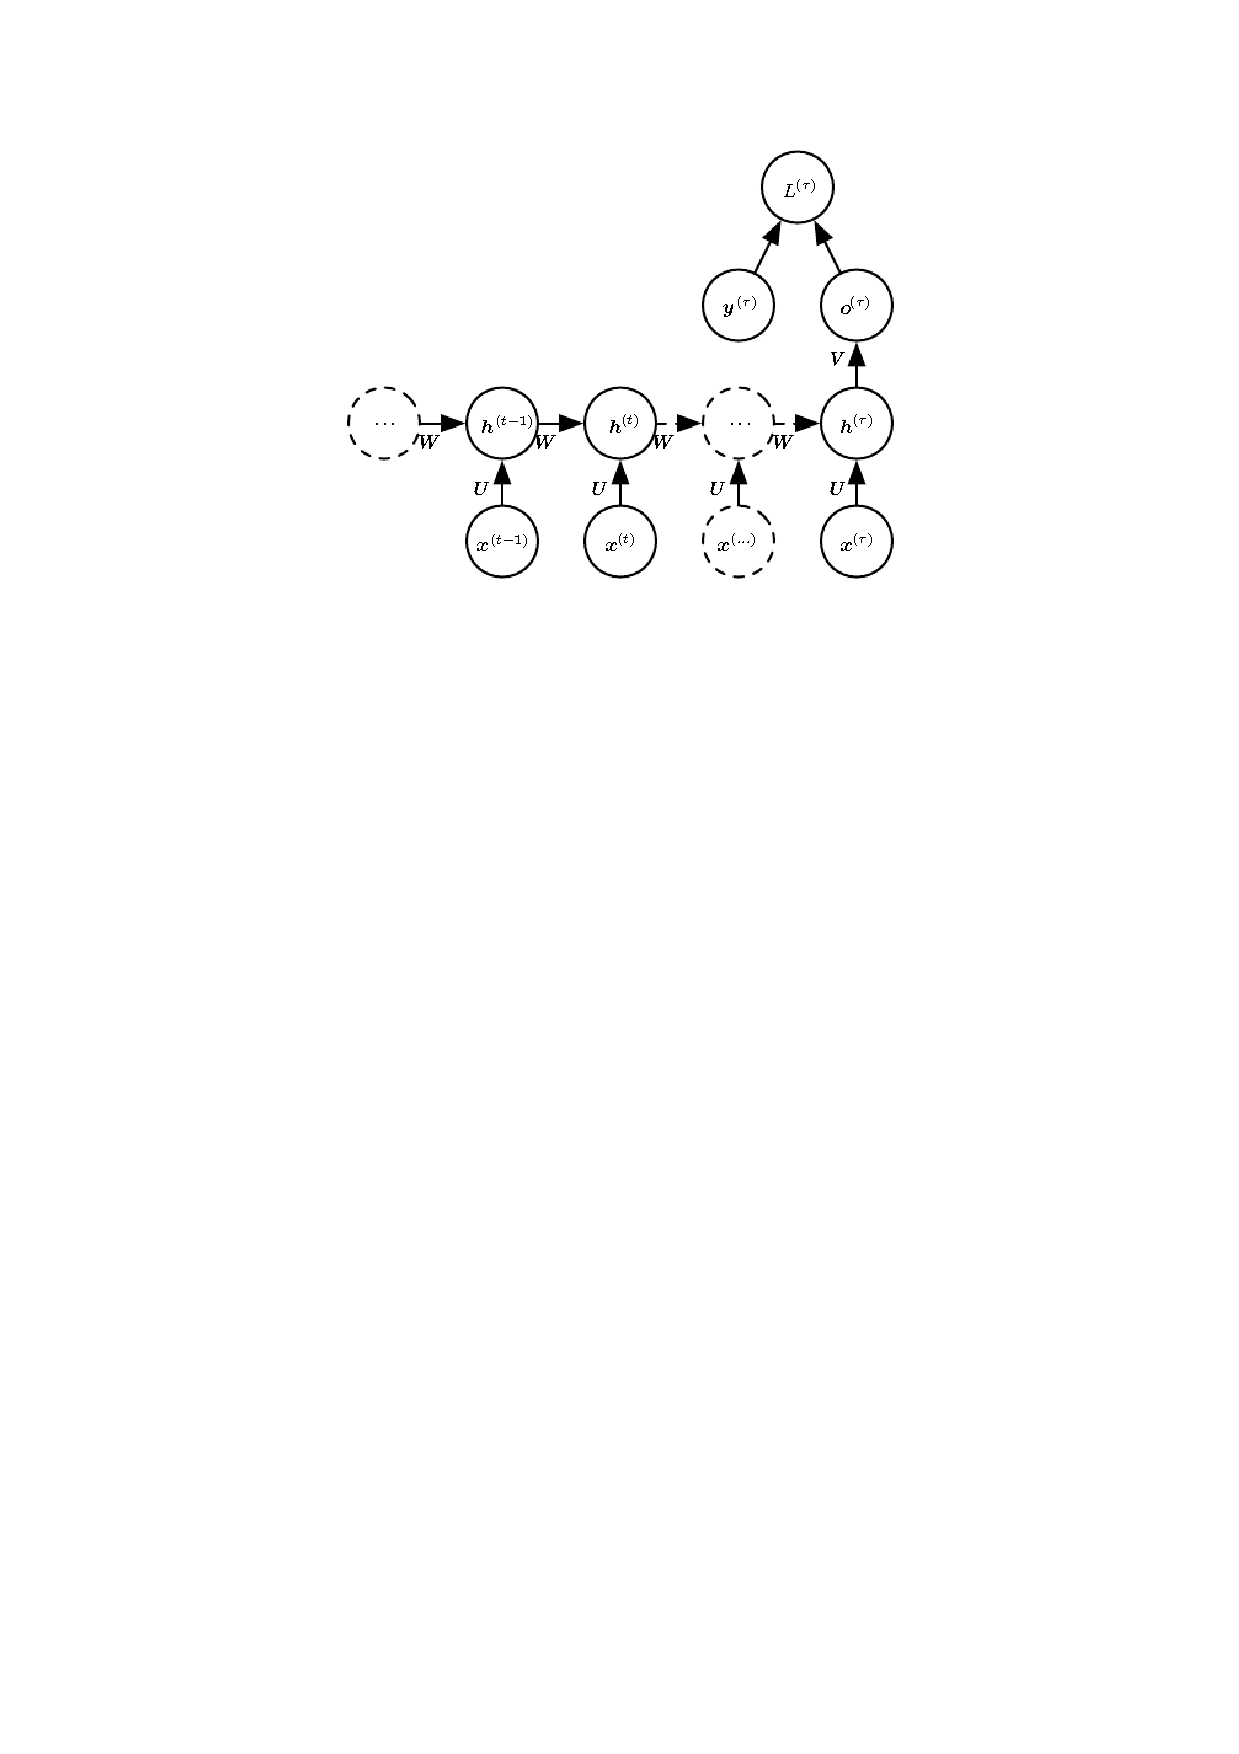
\includegraphics[width=0.9\textwidth]{../imgs/RNN_3.pdf}
\end{center}
\paragraph{Characteristics}
\begin{itemize}
    \item There might be a target right at the end, or the gradient on the ouput $\egvo{t}$ can be obtained by back-propagating from further downstream modules.
\end{itemize}
\paragraph{Applications}
\begin{enumerate}
    \item Summarize a sequence and produce a fixed-size representation used as input for further processing.
\end{enumerate}


\subsection{}
\begin{center}
    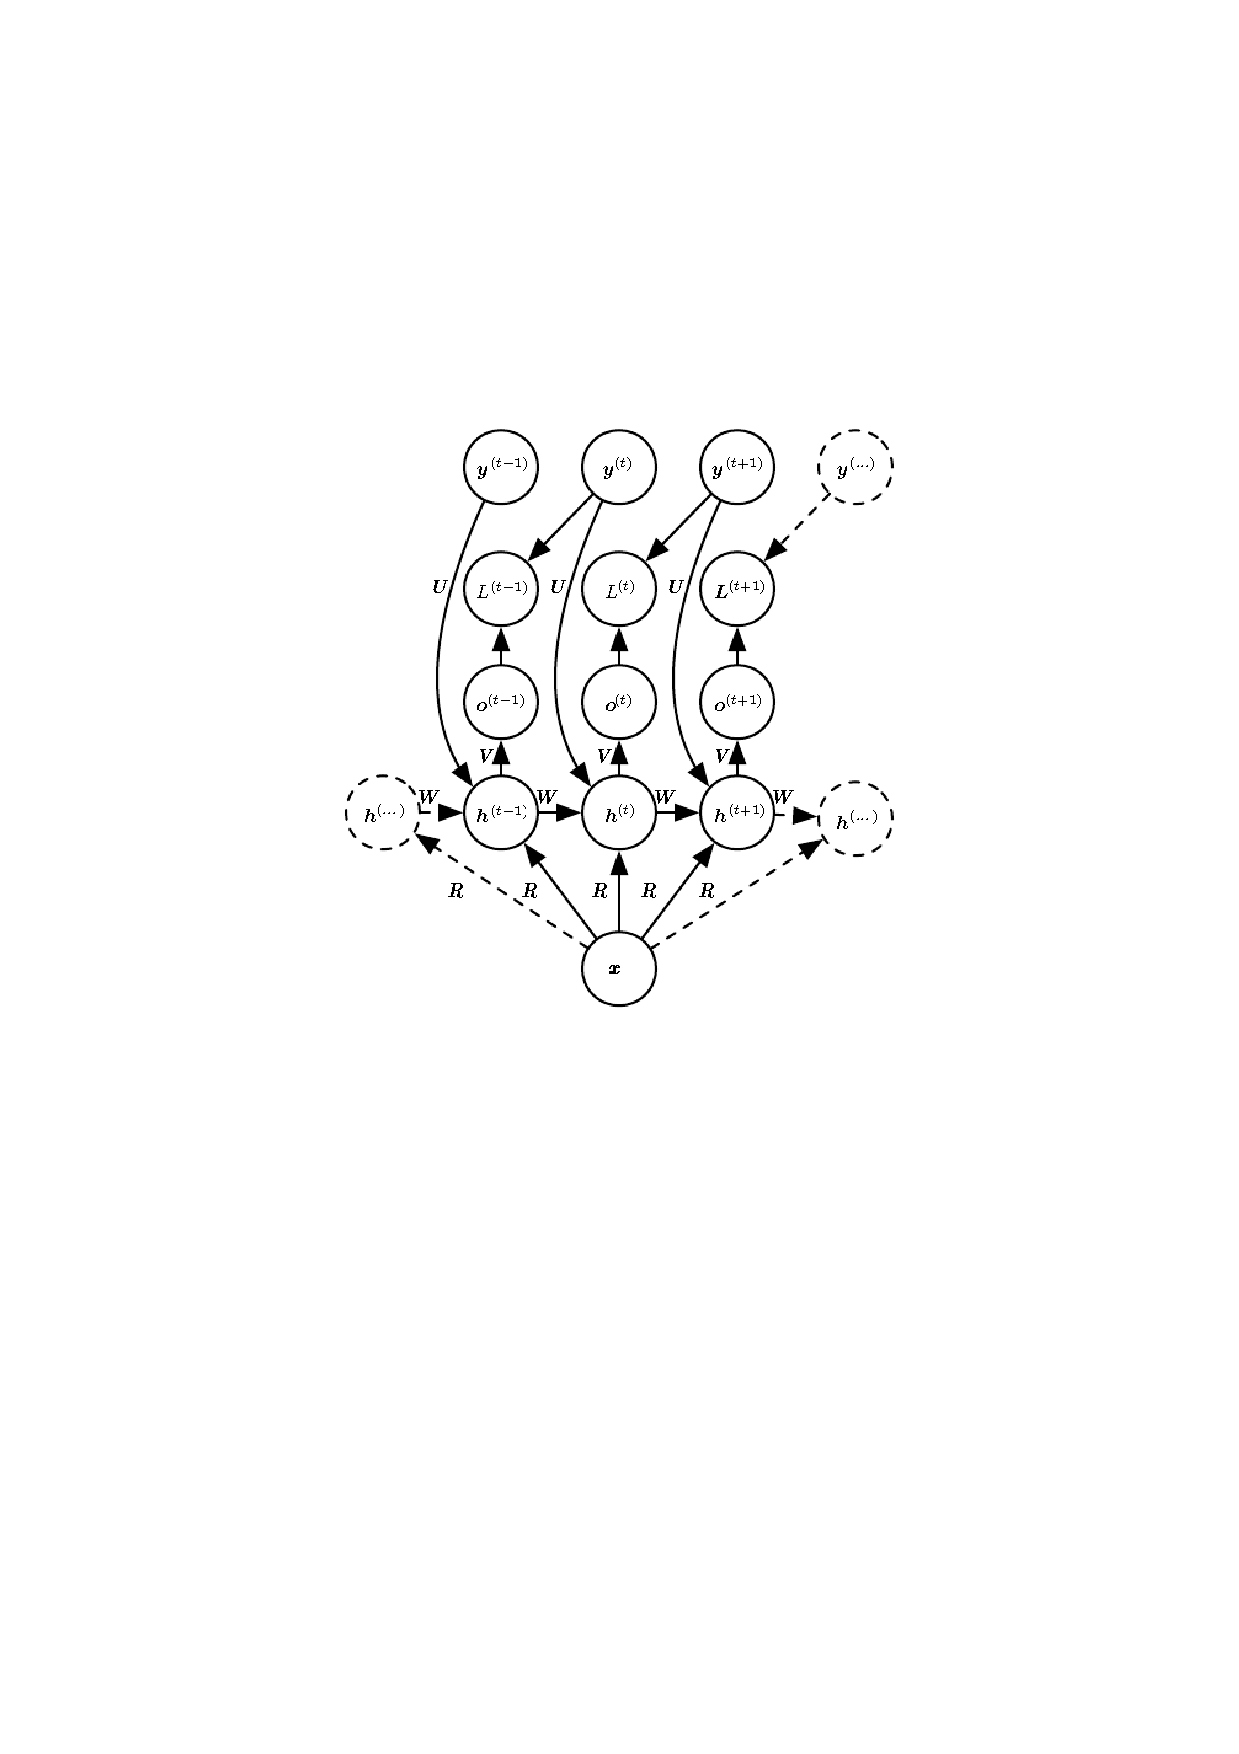
\includegraphics[width=0.9\textwidth]{../imgs/RNN_4.pdf}
\end{center}
\paragraph{Characteristics}
\begin{itemize}
    \item $\vx^\top \vR$ is effectively a new bias parameter.
    \item Each element $\egvy{t}$ of the observed output sequence serves both as input (for the current time step) and, during training, as target (for the previous time step).
\end{itemize}
\paragraph{Applications}
\begin{enumerate}
    \item Image captioning, where a single image is used as input to a model that then produces a sequence of words describing the image.
\end{enumerate}


\subsection{}
\begin{center}
    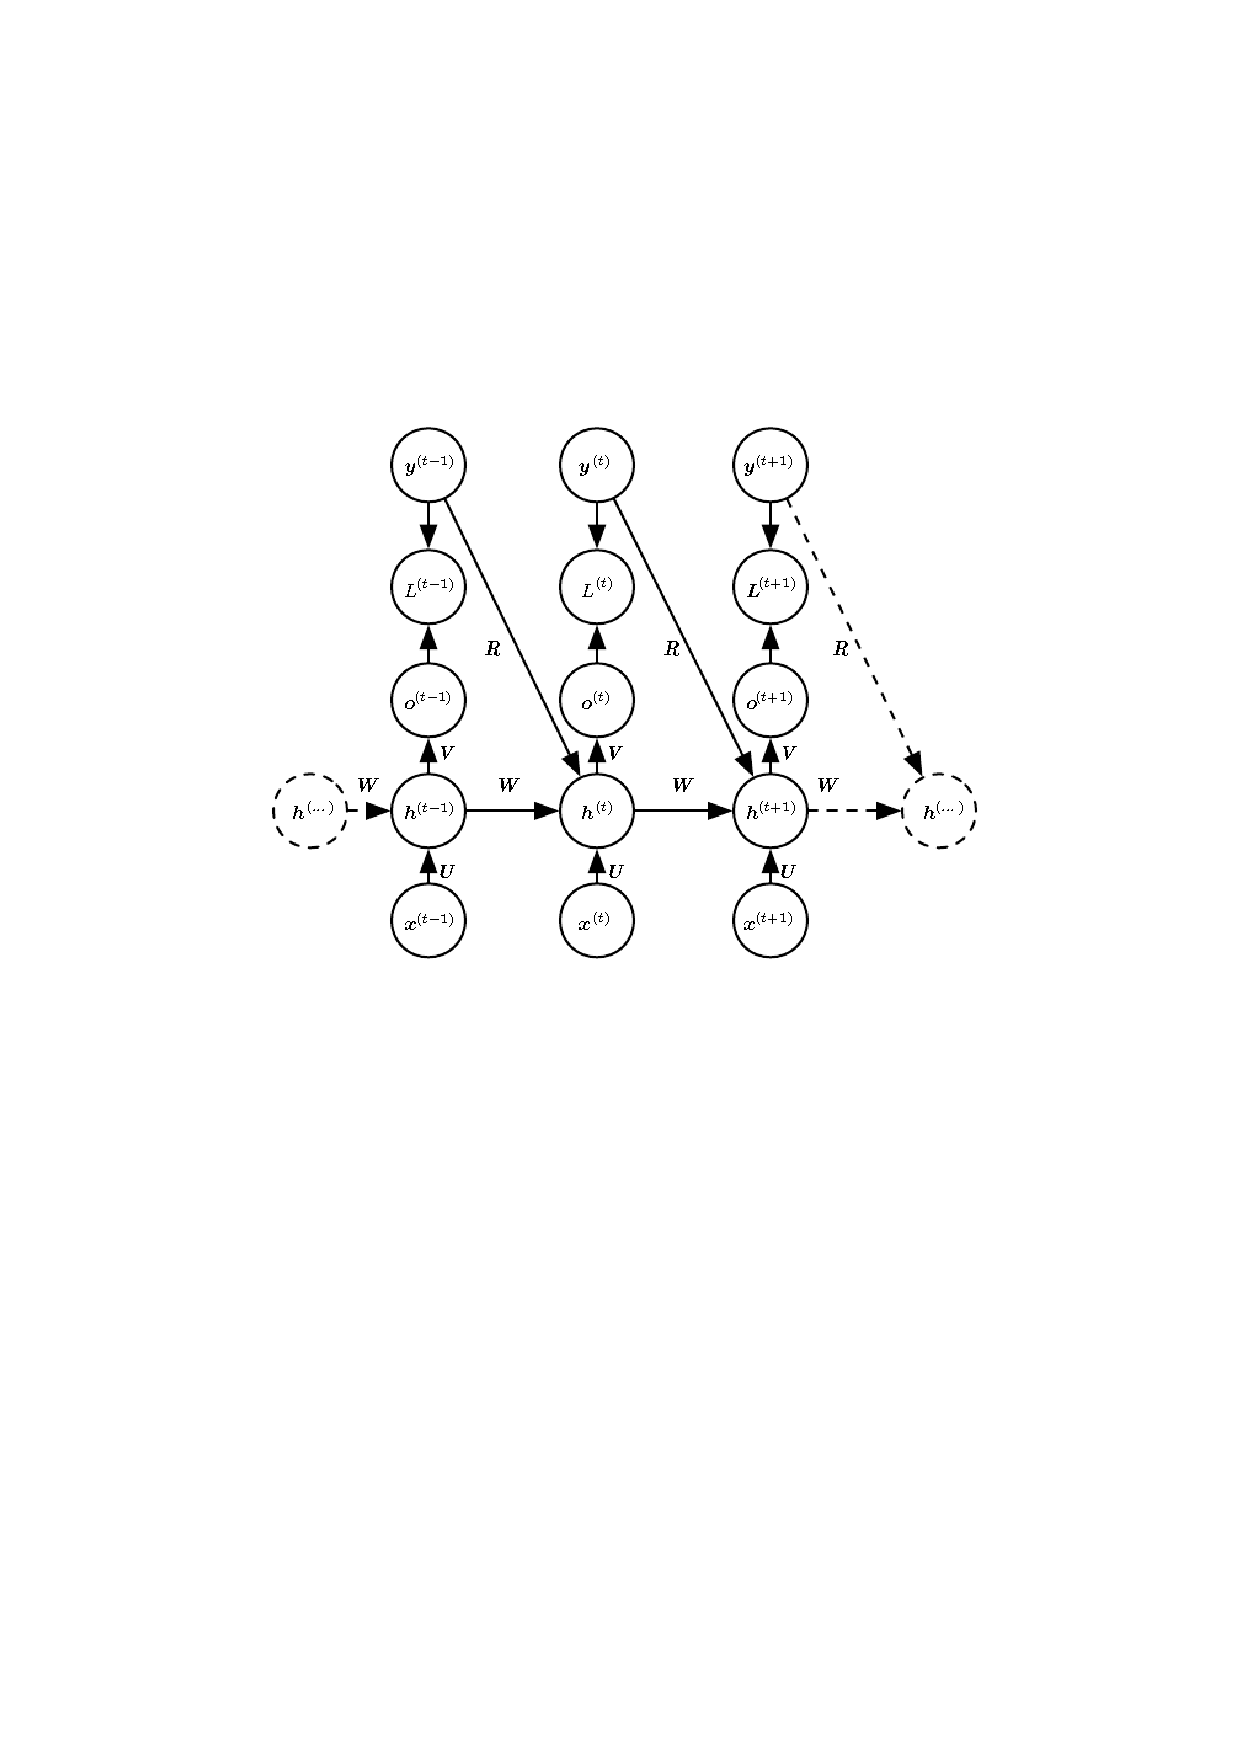
\includegraphics[width=0.9\textwidth]{../imgs/RNN_5.pdf}
\end{center}
\paragraph{Characteristics}
\begin{itemize}
    \item Because of connections from the output at time $t$ to the hidden unit at time $t+1$, the model can represent arbitrary probability distributions over the $\vy$ sequence (no conditional independence assumption).
\end{itemize}
\paragraph{Restrictions}
\begin{enumerate}
    \item The length of both sequences must be the same.
\end{enumerate}


\section{Back Propagation Through Time (BPTT)}
Here we talk about the BPTT of equation \ref{rnn_for} as forward propagation and equation \ref{rnn_loss} as loss function.
(Note: here $\eghvy{t} = \softmax(\egvo{t})$)
\begin{enumerate}
    \item $\displaystyle \pard{L}{\egL{t}} = 1$
    \item $\displaystyle \left( \nabla_{\egvo{t}} L \right)_i 
        = \pard{L}{\ego{t}_i} 
        = \pard{L}{\egL{t}} \pard{\egL{t}}{\ego{t}_i} 
        = \eghy{t}_i - \mathbbm{1}_{i=\egy{t}}$
    \item For $t=\tau$
        \[
            \nabla_{\egvh{\tau}}L = \vV^\top \nabla_{\egvo{\tau}} L  
        \]
        $\forall t = 1,\dots,\tau-1$
        \[
            \begin{split}
                \nabla_{\egvh{t}}L 
                &= \left( \pard{\egvh{t+1}}{\egvh{t}} \right)^\top (\nabla_{\egvh{t+1}}L) 
                + \left( \pard{\egvo{t}}{\egvh{t}} \right)^\top (\nabla_{\egvo{t}}L)
                \\&= \vW^\top \diag\left( 1-\left(\egvh{t+1}\right)^2 \right)(\nabla_{\egvh{t+1}}L) + \vV^\top(\nabla_{\egvo{t}}L)
            \end{split}
        \]
    \item
        \[
            \begin{split}
                \nabla_{\vc}L &\quad=\quad \sum_t\tpard{\egvo{t}}{\egvc{t}} \nabla_{\egvo{t}}L = \sum_t \nabla_{\egvo{t}}L
                \\ \nabla_{\vb}L &\quad=\quad \sum_t\tpard{\egvh{t}}{\egvb{t}} \nabla_{\egvh{t}}L = \sum_t \diag\left(1-\left(\egvh{t}\right)^2\right) \nabla_{\egvh{t}} L
                \\ \nabla_{\vV}L &\quad=\quad \sum_t\sum_i \pard{L}{\ego{t}_i} \nabla_{\egvV{t}} \ego{t}_i = \sum_t (\nabla_{\egvo{t}}L) {\egvh{t}}^\top
                \\ \nabla_{\vW}L &\quad=\quad \sum_t\sum_i \pard{L}{\egh{t}_i} \nabla_{\egvW{t}}\egh{t}_i
                \\&\quad=\quad \sum_t \diag\left(1 - \left(\egvh{t}\right)^2\right) (\nabla_{\egvh{t}} L) {\egvh{t-1}}^\top
                \\ \nabla_{\vU}L &\quad=\quad \sum_t\sum_i \pard{L}{\egh{t}_i} \nabla_{\egvU{t}}\egh{t}_i
                \\&\quad=\quad \sum_t \diag\left(1 - \left(\egvh{t}\right)^2\right) (\nabla_{\egvh{t}} L) {\egvx{t}}^\top
            \end{split}
        \]
\end{enumerate}


\section{Bidirectional RNNs}



\end{document}